\documentclass[conference]{IEEEtran}
\IEEEoverridecommandlockouts

\usepackage[utf8]{inputenc}
\usepackage[T1]{fontenc}
\usepackage{cite}
\usepackage{amsmath,amssymb,amsfonts}
\usepackage{graphicx}
\usepackage{textcomp}
\usepackage{xcolor}
\usepackage{url}
\usepackage{array}
\usepackage{placeins}
\usepackage{float}

\setlength{\textfloatsep}{6pt plus 1pt minus 2pt}
\setlength{\floatsep}{6pt plus 1pt minus 2pt}
\setlength{\intextsep}{6pt plus 1pt minus 2pt}

\newcommand{\placeholderbox}[2]{%
\fbox{\begin{minipage}[c][#1][c]{0.44\textwidth}\centering\footnotesize #2\end{minipage}}}

\begin{document}

\title{Dynamic Direction of Arrival Tracking and Beamforming with Using IMM Kalman Filter}

\author{
\IEEEauthorblockN{Mehmet Burak ALTINTAŞ}
\IEEEauthorblockA{\textit{Department of Electrical and Electronics Engineering} \\
\textit{Marmara University} \\
Istanbul, Türkiye \\
burakmehmet@marun.edu.tr}
\and
\IEEEauthorblockN{Prof. Dr. Engin MAŞAZADE}
\IEEEauthorblockA{\textit{Project Advisor} \\
\textit{Department of Electrical and Electronics Engineering} \\
\textit{Marmara University} \\
Istanbul, Türkiye \\
engin.masazade@marmara.edu.tr}
}

\maketitle

\begin{abstract}
This paper presents a dynamic direction of arrival (DoA) tracking and adaptive beamforming system for jammer suppression using a two-channel ADALM-Pluto SDR platform. The system combines the MUSIC algorithm for DoA estimation, an Interacting Multiple Model (IMM) Kalman filter for dynamic angular tracking, and adaptive beamforming techniques for interference mitigation. In the absence of a jammer, the dominant MUSIC peak is interpreted as the signal of interest (SOI), and the IMM Kalman filter tracks the SOI direction while the MVDR beamformer is steered toward the estimated angle. When a stronger jammer is present, the dominant MUSIC peak corresponds to the jammer direction, and the IMM Kalman filter tracks the jammer instead of the SOI. In this mode, the SOI is assumed to be located at a known broadside direction of $0^\circ$, and an LCMV beamformer is used to preserve the SOI direction while imposing a spatial null toward the tracked jammer. When the jammer is removed, the system switches back to SOI tracking and MVDR beamforming. The proposed architecture demonstrates a practical estimation and beamforming framework for dynamic interference scenarios.
\end{abstract}

\begin{IEEEkeywords}
Direction of Arrival, MUSIC, IMM Kalman Filter, MVDR Beamforming, LCMV Beamforming, Jammer Suppression, ADALM-Pluto SDR.
\end{IEEEkeywords}

\section{Introduction}
Direction of arrival (DoA) estimation and adaptive beamforming are important techniques in wireless communication, radar, and electronic warfare systems. In practical receiver environments, the desired signal may be corrupted by intentional or unintentional interference sources. If the interference source is stronger than the signal of interest (SOI), conventional receiver operation may become unreliable. Therefore, estimating the angular position of dominant sources and applying spatial filtering methods are essential for robust reception.

In this project, a dynamic DoA tracking and adaptive beamforming system is developed using a two-channel ADALM-Pluto SDR platform based on the AD936x transceiver family \cite{ad9363}. The proposed system operates in two modes. In the no-jammer mode, the dominant received source is assumed to be the SOI. The MUSIC algorithm \cite{schmidt_music} estimates the SOI DoA, and an IMM Kalman filter \cite{blom_imm,barshalom_tracking} tracks its angular motion. The tracked direction is then used to steer an MVDR beamformer \cite{capon_mvdr}. In the jammer-present mode, a stronger jammer is transmitted from the second transmitter channel. Since the jammer becomes the dominant source, MUSIC estimates the jammer DoA, the IMM Kalman filter tracks the jammer, and an LCMV beamformer \cite{van_trees} preserves the known broadside SOI direction while nulling the jammer.

The main contribution of this work is the implementation of a mode-dependent estimation and beamforming chain in which the same MUSIC and IMM Kalman structure is used for different physical tracking objectives. The overall processing flow is shown in Fig.~\ref{fig:system_overview}.

\begin{figure}[!t]
\centerline{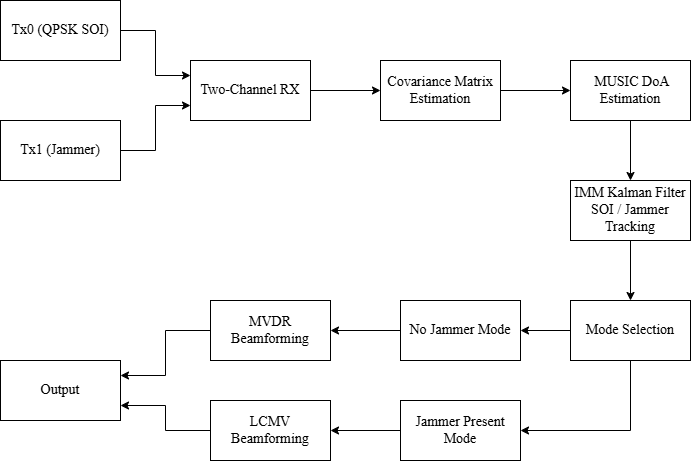
\includegraphics[width=0.48\textwidth]{Kalman_Project_Scheme.png}}
\caption{Overall processing flow of the proposed system with MUSIC-based DoA estimation, IMM Kalman tracking, and adaptive switching between MVDR and LCMV beamforming.}
\label{fig:system_overview}
\end{figure}

\section{System Model and Proposed Method}
\subsection{Signal and Array Model}
The receiver is modeled as a two-element uniform linear array (ULA) with inter-element spacing $d=\lambda/2$, where $\lambda$ is the wavelength at the carrier frequency. The broadside direction is defined as $0^\circ$. In the jammer-present mode, the SOI is assumed to arrive from broadside, while the jammer arrives from an arbitrary angle $\theta_j$, as illustrated in Fig.~\ref{fig:ula_geometry}.

\begin{figure}[!t]
\centerline{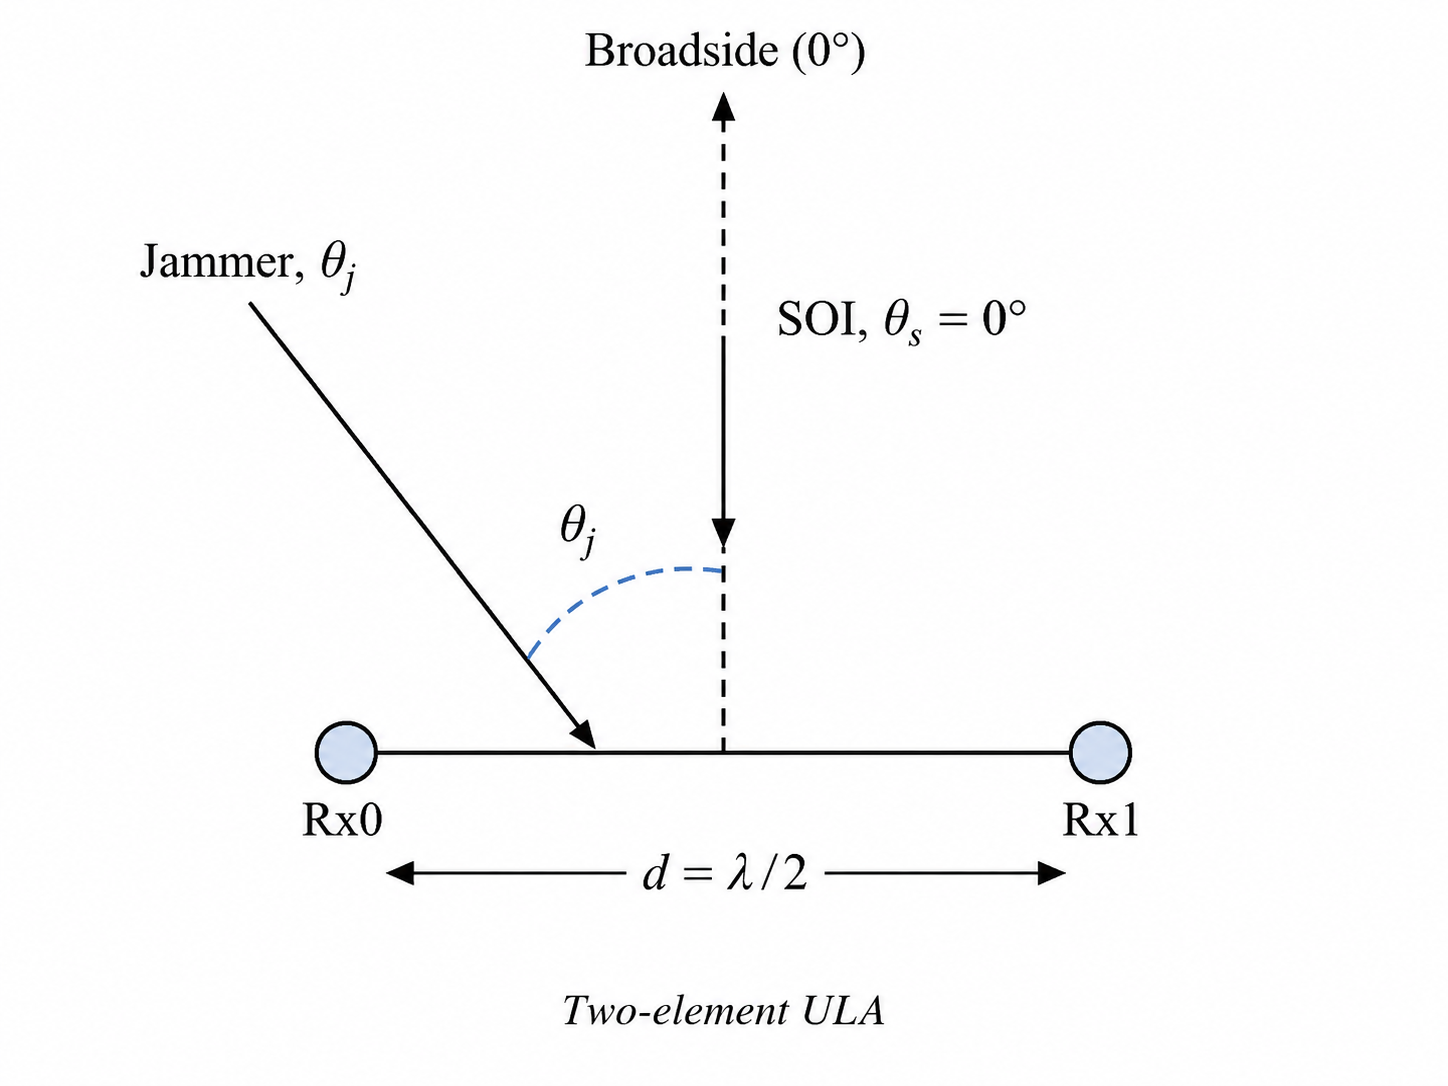
\includegraphics[width=0.42\textwidth]{ULA_Geometry.png}}
\caption{Two-element ULA geometry with broadside SOI direction and jammer direction.}
\label{fig:ula_geometry}
\end{figure}

For a plane wave arriving from angle $\theta$, the two-element steering vector is
\begin{equation}
\mathbf{a}(\theta)=
\begin{bmatrix}
1 & e^{-j2\pi \frac{d}{\lambda}\sin(\theta)}
\end{bmatrix}^{T}.
\label{eq:steering}
\end{equation}
The received array vector is modeled as
\begin{equation}
\mathbf{x}(n)=\mathbf{a}(\theta_s)s(n)+\mathbf{a}(\theta_j)j(n)+\mathbf{v}(n),
\label{eq:signal_model}
\end{equation}
where $s(n)$ is the QPSK SOI, $j(n)$ is the jammer, and $\mathbf{v}(n)$ is additive noise. In the no-jammer mode, the jammer term is absent. The spatial covariance matrix is estimated frame by frame as
\begin{equation}
\mathbf{R}_{xx}=\frac{1}{N}\sum_{n=1}^{N}\mathbf{x}(n)\mathbf{x}^{H}(n),
\label{eq:covariance}
\end{equation}
where $N$ is the number of IQ samples in one processing frame.

\subsection{MUSIC-Based DoA Estimation}
MUSIC estimates the dominant DoA by separating the signal and noise subspaces of $\mathbf{R}_{xx}$. After eigenvalue decomposition, the eigenvector associated with the smaller eigenvalue forms the noise subspace for the two-element, one-dominant-source case. The MUSIC pseudo-spectrum is
\begin{equation}
P_{\mathrm{MUSIC}}(\theta)=
\frac{1}{\mathbf{a}^{H}(\theta)\mathbf{E}_{n}\mathbf{E}_{n}^{H}\mathbf{a}(\theta)},
\label{eq:music}
\end{equation}
and the raw DoA measurement is obtained by
\begin{equation}
\hat{\theta}_{\mathrm{MUSIC}}=\arg\max_{\theta}P_{\mathrm{MUSIC}}(\theta).
\label{eq:music_peak}
\end{equation}
The scan range is selected as $-90^\circ$ to $+90^\circ$. Since the receiver has two antenna channels, MUSIC can reliably identify only one dominant source direction at a time. Thus, the same MUSIC output is interpreted as the SOI DoA in the no-jammer mode and as the jammer DoA in the jammer-present mode.

A practical two-element ULA may also exhibit mirror or image peaks, especially under phase calibration errors, IQ imbalance, finite snapshot effects, or multipath propagation. In jammer-present operation, selecting an image peak instead of the physical jammer direction may place the LCMV null inaccurately and degrade suppression. Therefore, phase calibration and interpretation of the dominant MUSIC peak are important for reliable operation.

\subsection{IMM Kalman Tracking}
The raw MUSIC estimate may fluctuate due to noise and covariance estimation errors. To obtain a smoother angular estimate, an IMM Kalman filter is used. The state vector is
\begin{equation}
\mathbf{x}_k=
\begin{bmatrix}
\theta_k & \dot{\theta}_k & \ddot{\theta}_k
\end{bmatrix}^{T},
\label{eq:imm_state}
\end{equation}
where $\theta_k$, $\dot{\theta}_k$, and $\ddot{\theta}_k$ are the angle, angular velocity, and angular acceleration. The measurement is the raw MUSIC DoA, $z_k=\hat{\theta}_{\mathrm{MUSIC},k}$, with measurement matrix $\mathbf{H}=\begin{bmatrix}1&0&0\end{bmatrix}$.

Three motion models are used in parallel: constant position (CP), constant velocity (CV), and constant acceleration (CA). For each model $i$, the Kalman prediction and update are
\begin{equation}
\hat{\mathbf{x}}_{k|k-1}^{(i)}=\mathbf{F}^{(i)}\hat{\mathbf{x}}_{k-1|k-1}^{(i)}, \quad
\mathbf{P}_{k|k-1}^{(i)}=\mathbf{F}^{(i)}\mathbf{P}_{k-1|k-1}^{(i)}\mathbf{F}^{(i)T}+\mathbf{Q}^{(i)},
\label{eq:kf_predict}
\end{equation}
\begin{equation}
\nu_k^{(i)}=z_k-\mathbf{H}\hat{\mathbf{x}}_{k|k-1}^{(i)}, \quad
\mathbf{K}_k^{(i)}=\mathbf{P}_{k|k-1}^{(i)}\mathbf{H}^{T}\left(S_k^{(i)}\right)^{-1},
\label{eq:kf_innov_gain}
\end{equation}
where $S_k^{(i)}=\mathbf{H}\mathbf{P}_{k|k-1}^{(i)}\mathbf{H}^{T}+R_k$. The innovation likelihood is used to update the model probability,
\begin{equation}
\mu_k^{(i)}=\frac{\Lambda_k^{(i)}\bar{\mu}_k^{(i)}}{\sum_{j=1}^{M}\Lambda_k^{(j)}\bar{\mu}_k^{(j)}},
\label{eq:model_probability}
\end{equation}
where $\bar{\mu}_k^{(i)}$ is the mixed/predicted model probability. The combined IMM estimate is
\begin{equation}
\hat{\mathbf{x}}_{k|k}=\sum_{i=1}^{M}\mu_k^{(i)}\hat{\mathbf{x}}_{k|k}^{(i)}, \quad
\hat{\theta}_{\mathrm{IMM},k}=\left[\hat{\mathbf{x}}_{k|k}\right]_1.
\label{eq:imm_output}
\end{equation}
The IMM filter switches between angular motion models, not between physical source identities. The physical meaning of the tracked angle is determined by the operating mode: SOI tracking in no-jammer operation and jammer tracking when the jammer is active.

\subsection{MVDR and LCMV Beamforming}
In the no-jammer mode, the IMM-filtered SOI direction $\hat{\theta}_{s}$ is used by the MVDR beamformer. MVDR minimizes the output power while preserving unity gain toward the desired direction:
\begin{equation}
\mathbf{w}_{\mathrm{MVDR}}=
\frac{\mathbf{R}_{xx}^{-1}\mathbf{a}(\hat{\theta}_{s})}{\mathbf{a}^{H}(\hat{\theta}_{s})\mathbf{R}_{xx}^{-1}\mathbf{a}(\hat{\theta}_{s})}.
\label{eq:mvdr}
\end{equation}
When the jammer is active, the SOI is assumed to be located at $\theta_s=0^\circ$, and the IMM output is interpreted as the jammer direction $\hat{\theta}_j$. The LCMV constraint matrix and response vector are
\begin{equation}
\mathbf{C}=\begin{bmatrix}\mathbf{a}(\theta_s)&\mathbf{a}(\hat{\theta}_j)\end{bmatrix}, \quad
\mathbf{f}=\begin{bmatrix}1&0\end{bmatrix}^{T}.
\label{eq:lcmv_constraints}
\end{equation}
The LCMV weights are
\begin{equation}
\mathbf{w}_{\mathrm{LCMV}}=\mathbf{R}_{xx}^{-1}\mathbf{C}\left(\mathbf{C}^{H}\mathbf{R}_{xx}^{-1}\mathbf{C}\right)^{-1}\mathbf{f}.
\label{eq:lcmv}
\end{equation}
Thus, the SOI direction is preserved while a spatial null is placed toward the tracked jammer.

\FloatBarrier
\section{Experimental Setup}
The experimental system is implemented using the ADALM-Pluto SDR platform. Tx0 transmits the QPSK SOI, and Tx1 transmits a CW jammer. The receiver uses two channels and processes IQ samples in real time. The SOI transmit gain is set to $-20$ dB, and the jammer gain is set to $-3$ dB. Therefore, the jammer is approximately 17 dB stronger than the SOI at the transmitter side under similar channel and antenna conditions.

Fig.~\ref{fig:experimental_setup} shows the SDR setup. The main parameters are summarized in Table~\ref{tab:params}.

\begin{figure}[H]
\centering
\IfFileExists{Experimental_Setup.jpeg}{%
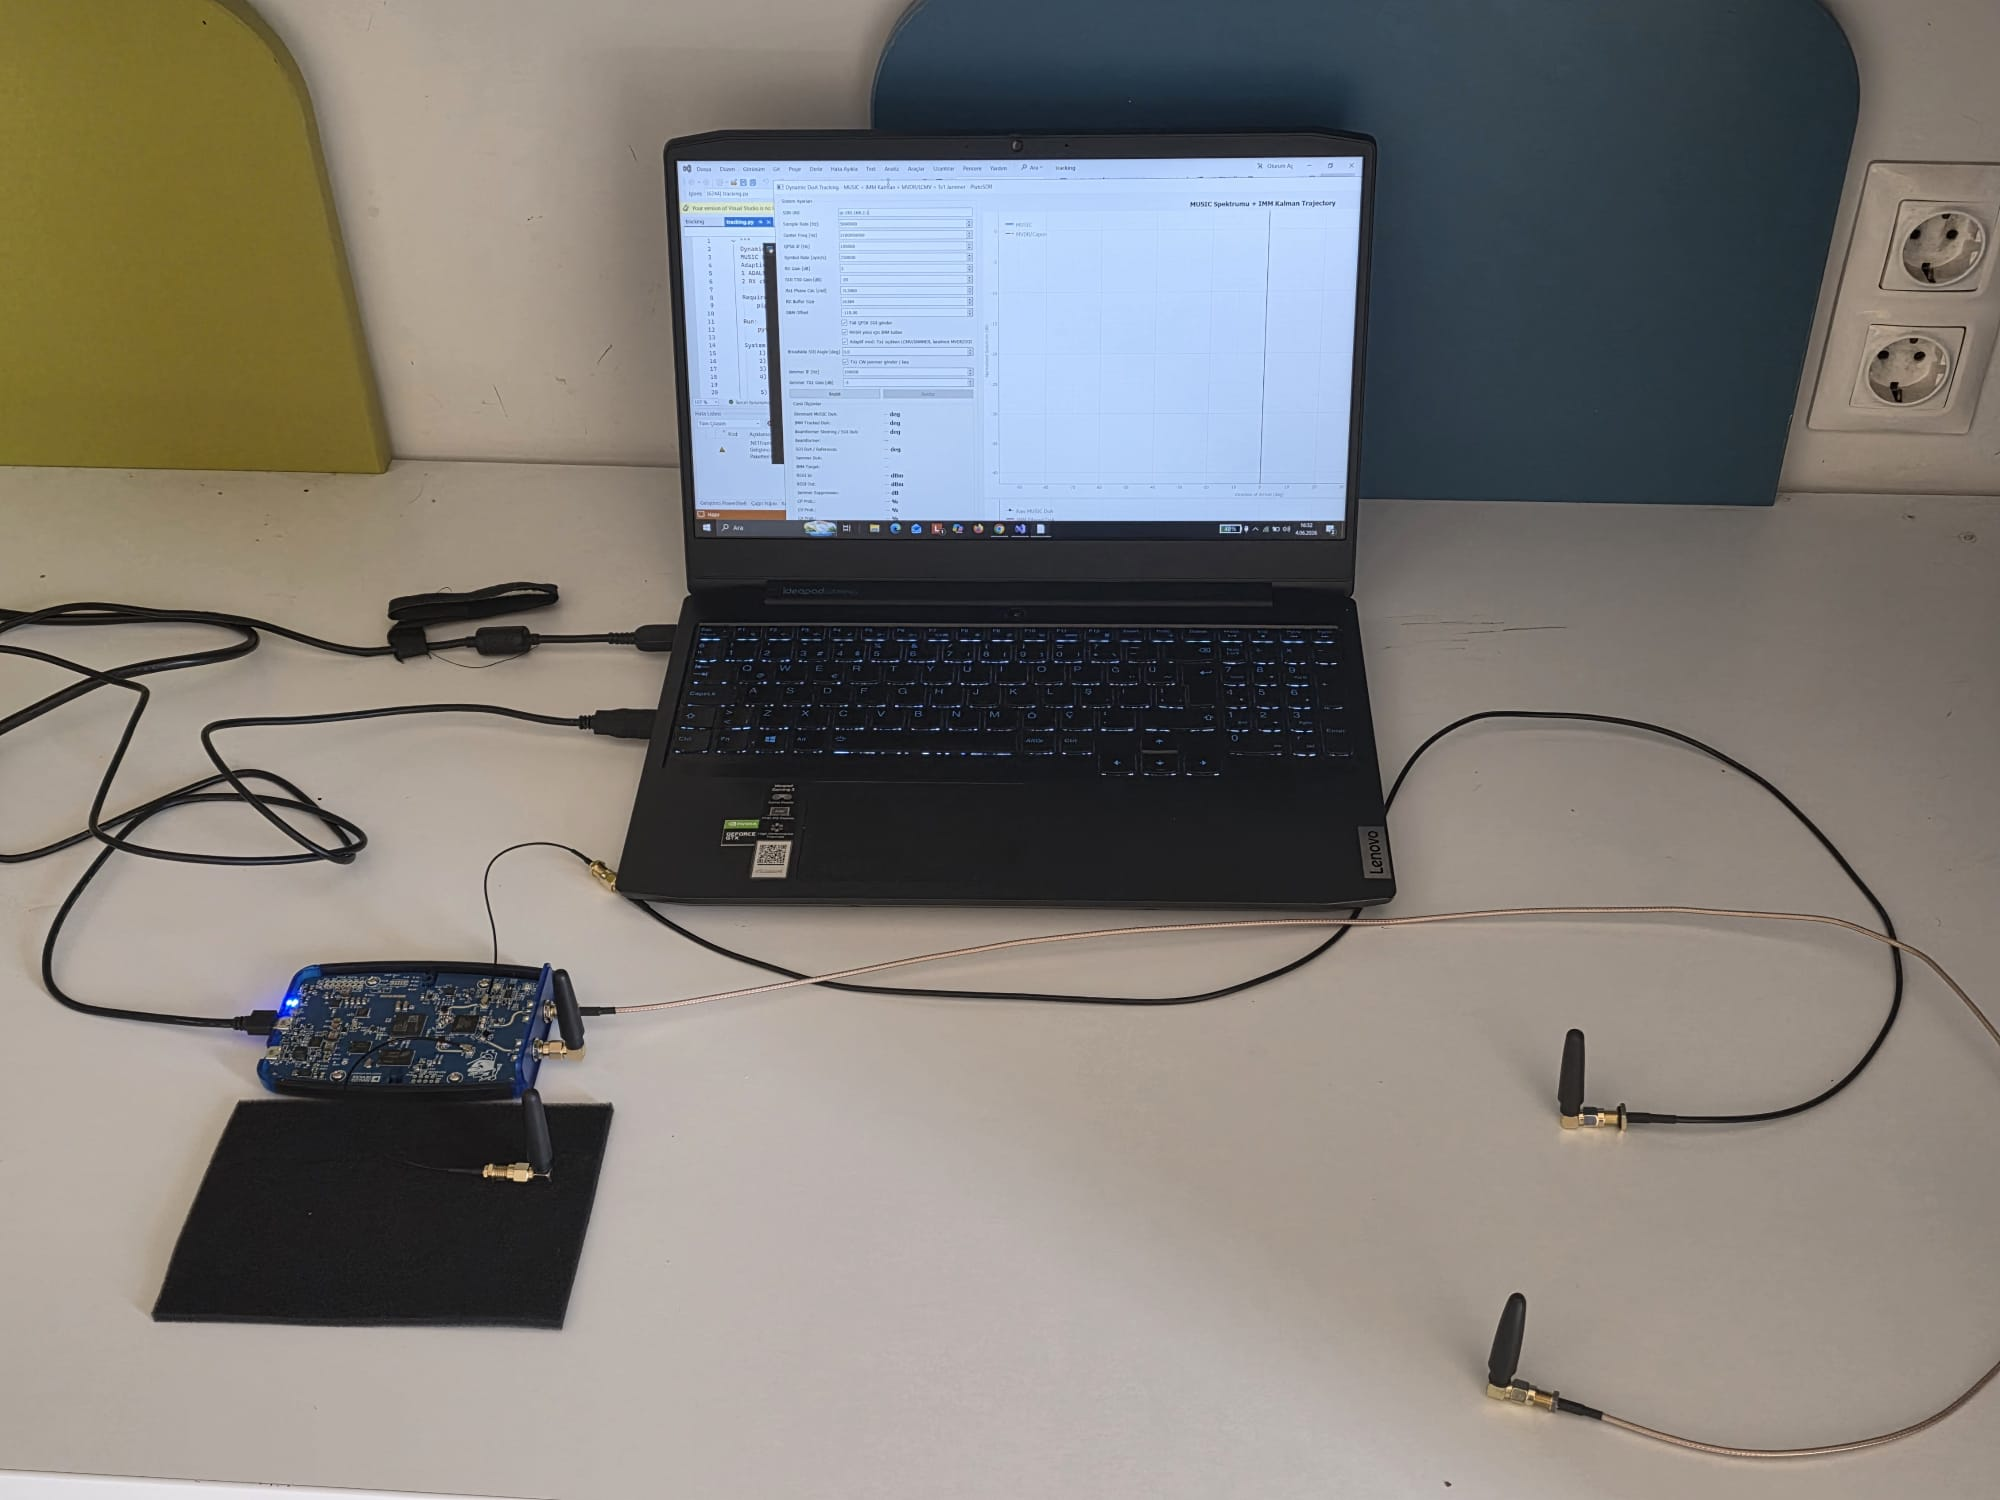
\includegraphics[width=0.48\textwidth]{Experimental_Setup.jpeg}%
}{%
\placeholderbox{3.0cm}{Experimental setup photo will be inserted here.\\ Add the file named Experimental\_Setup.jpeg to use the actual setup photo.}%
}
\caption{Experimental setup using the ADALM-Pluto SDR platform with Tx0 as the QPSK SOI source, Tx1 as the jammer source, and two receiver channels.}
\label{fig:experimental_setup}
\end{figure}

\begin{table}[H]
\caption{Experimental System Parameters}
\label{tab:params}
\centering
\footnotesize
\begin{tabular}{|>{\raggedright\arraybackslash}p{0.25\textwidth}|>{\raggedright\arraybackslash}p{0.17\textwidth}|}
\hline
\textbf{Parameter} & \textbf{Value} \\
\hline
SDR Platform & ADALM-Pluto / AD936x \\
RX Channels & 2 \\
RX Antenna Spacing & $d = \lambda/2$ \\
SOI / Jammer TX & Tx0 / Tx1 \\
Center Frequency & 2.1 GHz \\
Sampling Rate & 5 MS/s \\
SOI Modulation & QPSK \\
SOI / Jammer TX Gain & $-20$ dB / $-3$ dB \\
Jammer Type & CW Tone \\
DoA Scan Range & $-90^\circ$ to $+90^\circ$ \\
SOI Direction in Jammer Mode & $0^\circ$ \\
Beamformers & MVDR / LCMV \\
Tracking Filter & IMM Kalman \\
\hline
\end{tabular}
\end{table}



\subsection{Implementation Procedure and Evaluation Metrics}
The real-time implementation follows a frame-based processing structure. At each frame, the two-channel receiver buffer is acquired from the SDR and converted into a complex array data matrix. A fixed inter-channel phase calibration is applied before covariance estimation in order to reduce the effect of receiver-chain mismatch. The sample mean of each channel is removed, and the covariance matrix is computed from the calibrated frame. This covariance matrix is then used by the MUSIC estimator and by the selected adaptive beamformer.

The MUSIC spectrum is evaluated on a discrete angular grid between $-90^\circ$ and $+90^\circ$. The maximum of this spectrum provides the raw angular measurement for the IMM Kalman filter. In order to avoid abrupt steering changes caused by frame-to-frame fluctuations, the beamforming stage uses the IMM-filtered estimate rather than the raw MUSIC peak. The CP, CV, and CA model probabilities are updated at each frame according to the innovation likelihood, which allows the tracker to adapt to stationary and moving angular behavior without manually selecting a single motion model.

The operating mode determines how the filtered DoA is used. When the jammer is inactive, the filtered angle is treated as the SOI direction and MVDR beamforming is applied. When the jammer is active, the filtered angle is treated as the jammer direction, the SOI direction is fixed at broadside, and LCMV beamforming is applied. In the LCMV mode, diagonal loading is used in the covariance inversion stage to improve numerical robustness under finite-sample covariance estimates.

The main performance indicators are the raw MUSIC DoA, the IMM-filtered DoA, the selected beamformer mode, and the jammer suppression value. The suppression metric is evaluated only in the jammer-present LCMV mode, since it represents the reduction in output power associated with the active jammer. In no-jammer operation, this value is intentionally not reported because an input-output power difference would not correspond to interference suppression.


The mode-dependent processing logic is summarized as follows. If Tx1 is disabled, the receiver assumes that the dominant MUSIC peak belongs to the SOI and the IMM output is used as the steering direction. If Tx1 is enabled, the receiver assumes that the dominant MUSIC peak belongs to the jammer, because the jammer transmit gain is intentionally higher than the SOI transmit gain. In this case, the IMM output is used as the nulling direction. This explicit mode information avoids trying to classify two simultaneous sources from only two receiver channels, which would not be reliable for the considered array size.

A practical point in the implementation is that the DoA estimate is not only a display variable but also a control input for the beamformer. Therefore, a noisy DoA estimate can immediately affect the beamformer response. For this reason, the IMM output is used in the beamforming path. The raw MUSIC result is still displayed and stored because it shows the measurement quality and makes it possible to compare the Kalman-filtered trajectory with the unfiltered angular estimate. This comparison is especially important for the course objective, since it demonstrates the role of Bayesian filtering in stabilizing a measurement-driven receiver.

The suppression value is computed as the difference between the estimated input power and the beamformed output power during jammer-present operation. Although this value is not identical to output SINR improvement, it is a useful experimental indicator for observing the effect of the LCMV null. In the final measurements, this value will be interpreted together with the MUSIC spectrum, the tracked jammer direction, and the beam pattern response. A large suppression value without correct DoA tracking would not be meaningful; therefore, tracking consistency and null placement are evaluated together.

The implementation also includes practical safeguards. The covariance matrix is loaded before inversion to reduce sensitivity to finite-sample errors and ill-conditioned data. The DoA scan is limited to the visible angular region of the ULA, and the IMM angle state is bounded to prevent unrealistic angular jumps. These precautions do not change the theoretical structure of MUSIC, IMM, MVDR, or LCMV, but they improve the stability of the real-time demonstration.


\section{Results and Performance Evaluation}
This section presents the experimental results of the proposed adaptive DoA tracking and beamforming system. The results are evaluated in two main operating conditions: no-jammer operation and jammer-present operation. The mode switching and nulling response subsection is omitted in the final report because the main objective is sufficiently demonstrated by the individual SOI-tracking and jammer-tracking cases.

\subsection{No-Jammer Case}
In the no-jammer case, Tx1 is disabled and only the QPSK SOI is transmitted from Tx0. Under this condition, the dominant MUSIC peak corresponds to the SOI direction. The IMM Kalman filter tracks the SOI DoA, and the MVDR beamformer uses the IMM-filtered angle as the steering direction. Fig.~\ref{fig:no_jammer_result} shows the no-jammer result, including the MUSIC spectrum and the comparison between the raw MUSIC trajectory and the IMM-filtered trajectory.

\begin{figure}[!htbp]
\centerline{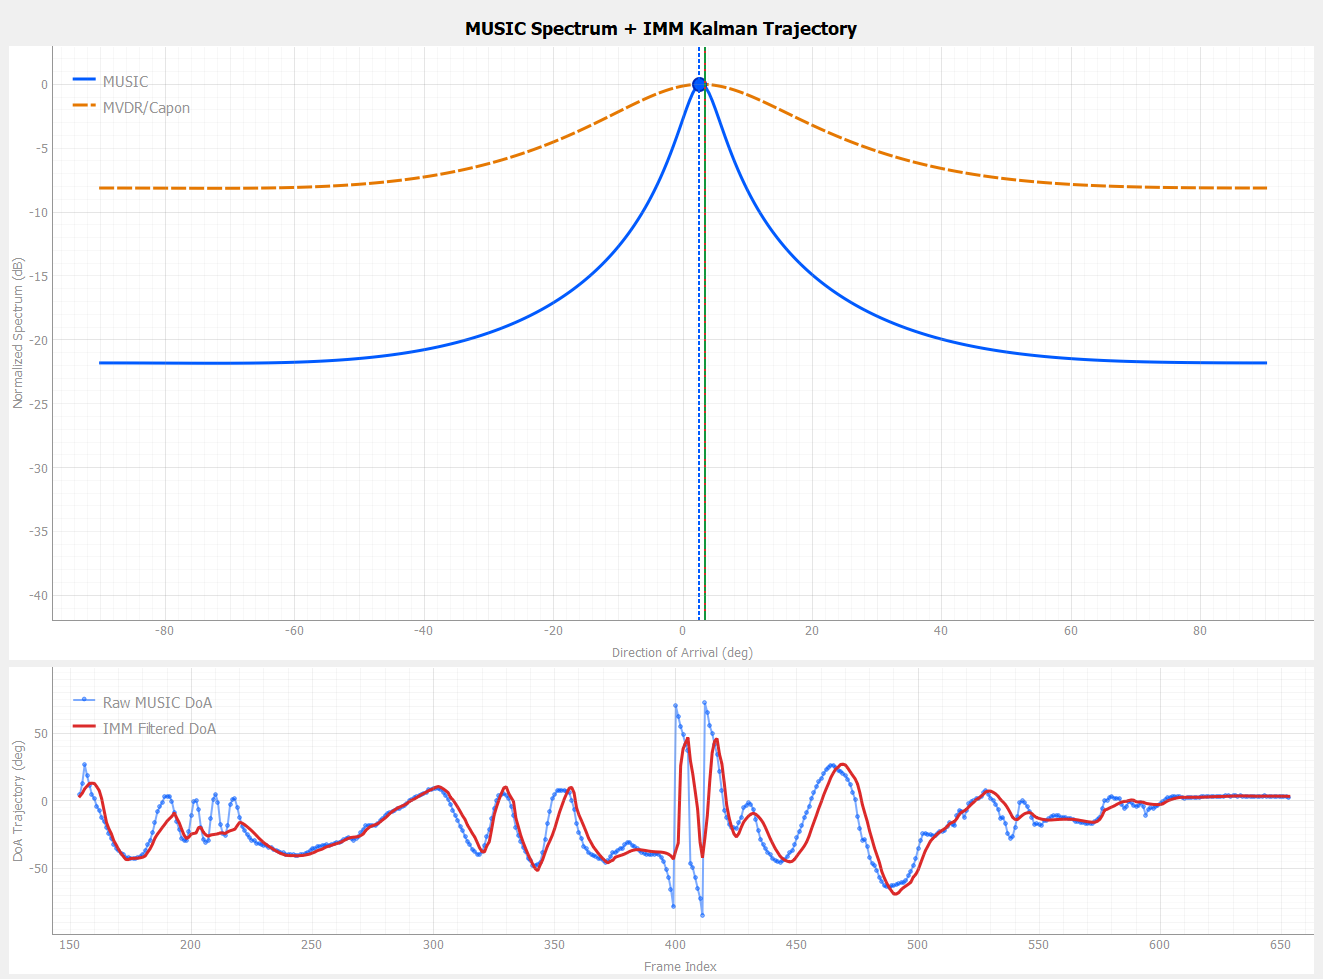
\includegraphics[width=0.48\textwidth]{no_jammer_result.png}}
\caption{No-jammer case: MUSIC spectrum showing the SOI DoA peak and comparison of raw MUSIC tracking with IMM-filtered SOI tracking.}
\label{fig:no_jammer_result}
\end{figure}

The result shows that the dominant DoA is associated with the SOI when the jammer is disabled. The raw MUSIC trajectory exhibits frame-to-frame fluctuations, while the IMM Kalman output provides a smoother angular trajectory. This filtered output is therefore more suitable as a control input for MVDR steering than the raw MUSIC peak.

\FloatBarrier

\subsection{Jammer-Present Case}
In the jammer-present case, Tx1 transmits the CW jammer while Tx0 continues transmitting the QPSK SOI. Since the jammer transmit gain is 17 dB higher than the SOI gain, the jammer becomes the dominant source in the received covariance matrix. Therefore, the MUSIC peak is interpreted as the jammer direction. The IMM Kalman filter tracks this jammer direction, while the SOI direction is kept fixed at broadside, $0^\circ$. The LCMV beamformer then preserves the SOI direction and places a null toward the tracked jammer. Fig.~\ref{fig:jammer_present_result} shows the jammer-present MUSIC spectrum and the jammer tracking behavior.

\begin{figure}[!htbp]
\centerline{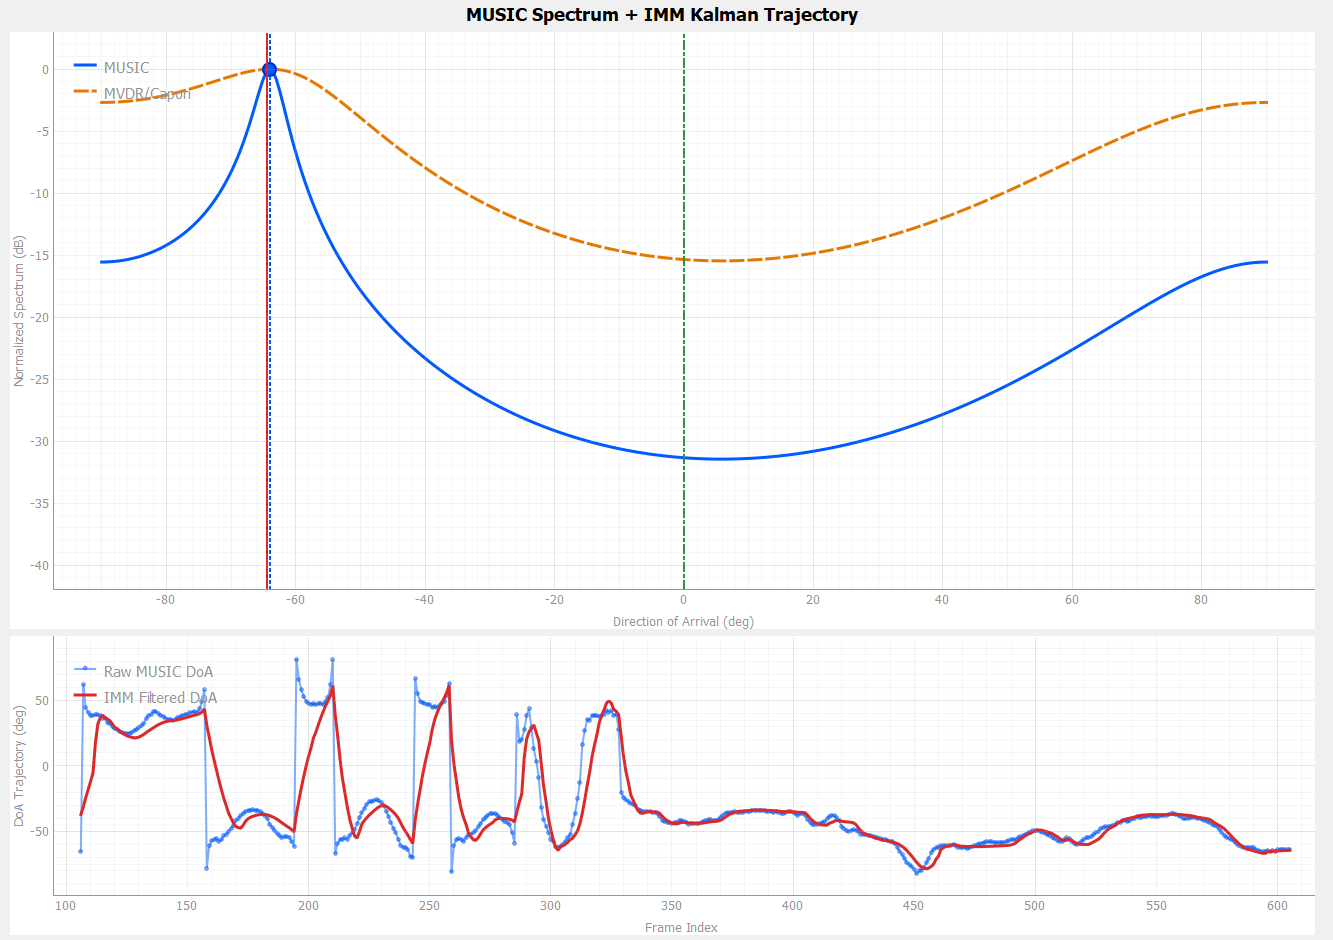
\includegraphics[width=0.48\textwidth]{jammer_present_result.png}}
\caption{Jammer-present case: MUSIC spectrum showing the jammer DoA peak and comparison of raw MUSIC tracking with IMM-filtered jammer tracking.}
\label{fig:jammer_present_result}
\end{figure}

The measured GUI values for the jammer-present case are shown in Fig.~\ref{fig:jammer_present_meas}. The dominant MUSIC DoA is measured as $-66.50^\circ$, while the IMM-filtered jammer DoA is $-68.42^\circ$. The beamformer operates in LCMV mode, the SOI reference is fixed at $0^\circ$, and the measured jammer suppression is $17.36$ dB. The input and output RSSI estimates are $-88.73$ dBm and $-106.10$ dBm, respectively.

\begin{figure}[!htbp]
\centerline{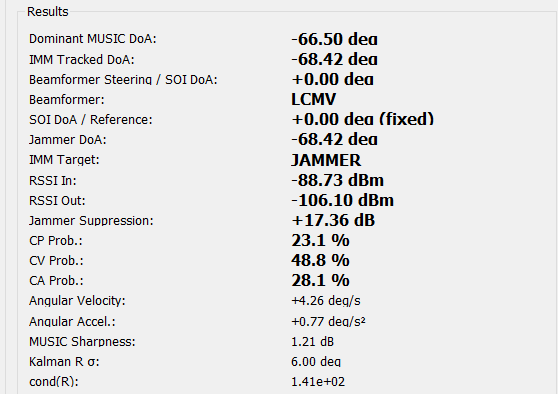
\includegraphics[width=0.34\textwidth]{jammer_present_meas.png}}
\caption{Measured parameters in the jammer-present case, including tracked jammer DoA, LCMV mode, RSSI values, and jammer suppression.}
\label{fig:jammer_present_meas}
\end{figure}

The suppression metric is evaluated only when the jammer is active and the beamformer operates in LCMV mode. When the jammer is disabled, this metric is not displayed because the input-output power difference would not represent actual jammer suppression. The measured 17.36 dB suppression indicates that the LCMV beamformer reduces the jammer-dominated received power while maintaining the broadside SOI constraint.

\FloatBarrier

The overall measured operating behavior is summarized in Table~\ref{tab:results_summary}.

\begin{table}[!htbp]
\caption{Summary of Measured Operating Modes}
\label{tab:results_summary}
\centering
\footnotesize
\begin{tabular}{|c|c|c|c|}
\hline
\textbf{Case} & \textbf{Beamformer} & \textbf{IMM Target} & \textbf{Suppression} \\
\hline
No Jammer & MVDR & SOI & -- \\
Jammer Active & LCMV & Jammer & 17.36 dB \\
\hline
\end{tabular}
\end{table}

\FloatBarrier

\section{Limitations and Discussion}
The main limitation of the proposed system is the use of only two receiver channels. With a two-element array, MUSIC can reliably estimate only one dominant source direction at a time. Therefore, the system cannot independently resolve the SOI and jammer directions when both are active. Instead, the dominant peak is interpreted according to the operating mode.

Another limitation is the broadside SOI assumption in the jammer-present mode. The LCMV beamformer assumes that the SOI is known and fixed at $0^\circ$. If the SOI moves while the jammer is active, additional receiver elements or a separate SOI tracking mechanism would be required. Moreover, phase mismatch, IQ imbalance, finite snapshot length, and multipath propagation may cause mirror peaks or steering vector errors. These effects can reduce DoA accuracy and degrade the LCMV null depth.

Finally, the nominal 17 dB transmitter gain difference does not necessarily represent the exact received jammer-to-SOI power ratio, because cable losses, antenna gains, coupling, and placement affect the received powers. Communication-level metrics such as output SINR, BER, and EVM can be added in later measurements to provide a more complete evaluation of SOI quality.

\section{Conclusion}
In this project, a dynamic DoA tracking and adaptive beamforming system was developed for jammer suppression using a two-channel ADALM-Pluto SDR platform. The proposed system combines MUSIC-based DoA estimation, IMM Kalman filtering, and mode-dependent adaptive beamforming. In the no-jammer mode, the dominant MUSIC peak is interpreted as the SOI direction, the IMM Kalman filter tracks the SOI, and MVDR beamforming is used. In the jammer-present mode, the stronger jammer becomes the dominant source, the IMM Kalman filter tracks the jammer, and LCMV beamforming preserves the known broadside SOI direction while placing a null toward the tracked jammer.

The architecture demonstrates how Bayesian tracking and adaptive array processing can be combined for dynamic interference mitigation. Although the current implementation is limited by the two-element array and the broadside SOI assumption, it provides a clear framework for receiver operation that adapts when a stronger interference source appears or disappears.


\section{Future Work}
The next stage of this work is to move the real-time processing chain from the host computer to the embedded processing resources of the ADALM-Pluto SDR. The PlutoSDR platform contains a Xilinx Zynq Z-7010 device with an ARM Cortex-A9 processing system and programmable logic resources. Therefore, the MUSIC, IMM Kalman tracking, and beamforming control loop can be migrated toward an embedded implementation in order to reduce the dependency on a host computer and to avoid continuous high-rate IQ streaming over USB.

In the first embedded implementation stage, the frame-based receiver processing can be executed on the ARM Cortex-A9 processor under the PlutoSDR embedded Linux environment. The main objective of this step is to keep the same algorithmic structure while moving covariance estimation, MUSIC peak search, IMM Kalman update, and mode-dependent beamformer selection into the SDR itself. This would enable a more self-contained receiver that can estimate the jammer direction and update the beamforming state locally.

In a later stage, computationally intensive operations can be accelerated on the Zynq Z-7010 programmable logic. Candidate hardware acceleration blocks include covariance accumulation, complex multiply-accumulate operations, beamformer output calculation, and repeated steering-vector evaluations over the DoA scan grid. Moving these operations to the FPGA fabric can reduce processing latency and make the system more suitable for real-time adaptive interference suppression. Fixed-point implementation, DMA-based data movement, and hardware/software partitioning will be important design considerations for this stage.

Future extensions may also include additional receiver channels, multi-jammer scenarios, and communication-level performance metrics such as output SINR, BER, and EVM. With more array elements, the system would be able to estimate multiple source directions simultaneously instead of relying on the dominant-source assumption used in the current two-channel implementation.

\begin{thebibliography}{00}
\bibitem{ad9363}
Analog Devices, ``AD9363 RF Agile Transceiver Data Sheet,'' Analog Devices.

\bibitem{schmidt_music}
R. O. Schmidt, ``Multiple emitter location and signal parameter estimation,'' \textit{IEEE Transactions on Antennas and Propagation}, vol. 34, no. 3, pp. 276--280, Mar. 1986.

\bibitem{capon_mvdr}
J. Capon, ``High-resolution frequency-wavenumber spectrum analysis,'' \textit{Proceedings of the IEEE}, vol. 57, no. 8, pp. 1408--1418, Aug. 1969.

\bibitem{van_trees}
H. L. Van Trees, \textit{Optimum Array Processing: Part IV of Detection, Estimation, and Modulation Theory}. New York, NY, USA: Wiley-Interscience, 2002.

\bibitem{stoica_moses}
P. Stoica and R. Moses, \textit{Spectral Analysis of Signals}. Upper Saddle River, NJ, USA: Prentice Hall, 2005.

\bibitem{barshalom_tracking}
Y. Bar-Shalom, X. R. Li, and T. Kirubarajan, \textit{Estimation with Applications to Tracking and Navigation: Theory, Algorithms and Software}. New York, NY, USA: Wiley, 2001.

\bibitem{blom_imm}
H. A. P. Blom and Y. Bar-Shalom, ``The interacting multiple model algorithm for systems with Markovian switching coefficients,'' \textit{IEEE Transactions on Automatic Control}, vol. 33, no. 8, pp. 780--783, Aug. 1988.
\end{thebibliography}

\end{document}
